\documentclass[conference]{IEEEtran}
\IEEEoverridecommandlockouts

\usepackage{cite}
\usepackage{amsmath,amssymb,amsfonts}
\usepackage{algorithmic}
\usepackage{graphicx}
\usepackage{textcomp}
\usepackage{mathtools}
\usepackage{csquotes}
\usepackage{cleveref}
\usepackage{verbatim}

\usepackage{tabularx,ragged2e,booktabs}

\def\BibTeX{{\rm B\kern-.05em{\sc i\kern-.025em b}\kern-.08em
    T\kern-.1667em\lower.7ex\hbox{E}\kern-.125emX}}

\hyphenation{}

\begin{document}

\title{Performance Enhancement and Security Analysis of Satellite FSO/QKD Systems using HAP-based Relaying and ARQ
}

\author{\IEEEauthorblockN{$\textnormal{Nam Nguyen}$}
\IEEEauthorblockA{$\textnormal{School of Electrical and Computer Engineering, Oregon State University, Corvallis, OR, 97331
}$\\
Email: \textnormal{nguynam4@oregonstate.edu}}
}

\maketitle
\begin{abstract}
This project proposes to use high-altitude platform (HAP)-based relaying and link-layer automatic repeat request (ARQ) techniques to improve the performance of satellite quantum key distribution (QKD) over free-space optics (FSO) systems. I also develop analytical frameworks based on two 3-D Markov chain models allowing to comprehensively analyze the proposed system's performance in terms of key loss rate and delay outage rate. For security analysis, ergodic secret-key rate is concisely derived. The performance analysis takes into account the physical layer impairments induced by free-space optical (FSO) channel and receiver noise. Numerical results quantitatively demonstrate that the satellite FSO/QKD system using HAP-based relaying and link-layer ARQ techniques can offer considerable performance improvement over the conventional ones. 
\end{abstract}

\renewcommand\IEEEkeywordsname{Keywords}
\begin{IEEEkeywords}
Quantum key distribution (QKD); High-altitude platform (HAP); Free-space optics (FSO); Automatic repeat request (ARQ); Key loss rate (KLR); Delay outage rate.
\end{IEEEkeywords}

\IEEEpeerreviewmaketitle

%=============================================================
\section{Introduction}
The desire of connecting everything over Internet requires the secure communication to prevent unauthorized access, stealing, and changing information. Quantum key distribution (QKD), a well-known protocol based on the rule of quantum physics to share the secret key via two lawful parties (namely Alice and Bob) with eavesdropper existed (namely Eve), is a promising method that meets the requirements \cite{Yuen2016}. A global-scale QKD network can be implemented utilizing satellite-to-ground free-space optical (FSO) links and several proof-of-principle experiments have been performed recently. However, the performance of satellite QKD systems is degraded by atmospheric channels including scattering, absorption, and atmospheric turbulence \cite{Vallone2015, Liao2018}. Due to these factors, even if there exists no eavesdropper existed, quantum key error rate (QKER) may be very high under strong turbulence. To reduce QKER, the reconciliation process based on forward error correction (FEC) has been proposed in \cite{Buttler2003} and further developed in \cite{Ai2020}. Nevertheless, highly computational algorithms are needed for optimizing FEC redundancy and, more importantly, FEC-only techniques are not robust enough to guarantee reliability due to relatively long-distance transmissions from satellite to ground stations (GSs). 

\begin{figure}[t]
\begin{center}
\includegraphics[width=0.9\columnwidth,height=.2\textheight]{Figures/Figure1.pdf}
\end{center}
\caption{Satellite FSO/QKD system using HAP-based relaying and link-layer ARQ techniques.}
\label{fig:Scheme}
\end{figure}

The main objective of this project is to explore additional techniques to improve performances of satellite FSO/QKD system shown in Fig. \ref{fig:Scheme}. I first strengthen the physical layer by considering a relaying technique based on a high-altitude platform (HAP). Here, a relaying node is located at a HAP that recovers the quantum keys transmitted from a satellite and forwards those keys to a ground station. Thanks to HAP-based relaying technique, the signal is regenerated and thus the QKER is reduced. Also, I improve the link layer by considering a key-retransmission technique, namely automatic repeat request (ARQ). Unlike FEC technique, which key errors are corrected based on the redundancy added to quantum keys to reduce QKER in the reconciliation process, link-layer ARQ technique retransmits unsuccessfully keys to assure QKD reliability. ARQ technique does not require high computational algorithms for error control; however, it may cause a high delay due to long transmission distance when keys are retransmitted from the satellite. To solve this problem, I propose to equip a buffer at HAP to store and retransmit the keys when needed. As the distance from HAP to GS is much smaller than the distance from the satellite to GS, the delay is reduced significantly. Finally, crucial performance metrics, including key loss rate and delay outage rate, can be analyzed for validating the feasibility of the proposed system. Selected numerical results demonstrate the performance metrics of proposed system are considerably improved compared to that of the conventional ones. 

\begin{figure*}[t]
\begin{center}
\includegraphics[width=12.3cm, height=4.7cm]{Figures/Figure2.pdf}
\end{center}
\caption{The proposed satellite FSO/QKD system using HAP-based relaying and link-layer ARQ techniques.}
\label{fig:SystemModel}
\end{figure*} 

The rest of this project is organized as follows. The proposed satellite FSO/QKD system using HAP-based relaying and link-layer ARQ techniques is described in Section \ref{sect:SystemModell}. In Section \ref{sect:PerformanceAnalysis}, performance analysis consists of key loss rate and delay outage rate is carried out. In Section \ref{sect:NumercialResults}, selected numerical results are presented. Finally, Section \ref{sect:Conclusion} concludes the project.

%=============================================================
\section{System Model}
\label{sect:SystemModell}
\subsection{QKD Protocol}
\label{QKD}
In this study, I employ continuous variable (CV)-QKD protocol due to its capability of providing high key generation rates and especially the compatibility with the standard optical communication technologies. Based on the CV-QKD protocol proposed in \cite{MinhVu2019}, Alice encodes the random sequences (i.e., quantum keys) using quadrature phase shift keying (QPSK) signaling and Bob uses dual-threshold (D-T) to detect the signal with the decision rule as
\begin{align}
\label{decision}
\textnormal{Decision}=\left\{\begin{matrix}
$0$ & \textnormal{if}~\left ( I\geq d_{0} \right )\\ 
$1$ & \textnormal{if}~\left ( I\leq d_{1} \right )\\ 
$X$ & \textnormal{otherwise}
\end{matrix}\right.
\end{align}
where $d_0$ and $d_1$ are two levels of the D-T which symmetrically selected via the \enquote{zero} level. Similar to the inaccurate bases choice in conventional BB84 protocol, \enquote{$X$} denotes that Bob does not retrieve Alice's transmitted bits \cite{Bennett1984}. Over a radio frequency (RF) public link, time instants when Bob can detect binary bits from received signals, are instantly informed to Alice. Accordingly, Alice also eliminates binary bits corresponds to time instants when Bob detects unidentified bits. Hence, a similar bit sequence is shared between Alice and Bob, is known as \textbf{\textit{sifted key}}. Because of detector/channel imperfections and/or eavesdropping, the sifted key may consist of errors. Similar step as in the original BB84, information reconciliation will be carried out to correct these errors and form error-free \textbf{\textit{secret key}}. However, instead of using FEC, the link-layer ARQ scheme is employed in our considered QKD system. 

\subsection{HAP-based Relaying Technique}
In Fig. \ref{fig:SystemModel}, the proposed satellite FSO/QKD system using HAP-based relaying and link-layer ARQ technique is described, including a satellite (Alice), a HAP-based relaying node (Ruby), and a ground station (Bob) which receives Ruby's optical signal to recover Alice's transmitter keys. I investigate the downlink transmission from Alice's transmitter placed on the satellite over Ruby's HAP to Bob's receiver placed on the ground station. Besides, a classical public channel is used for the link-layer ARQ feedback signal.

At the satellite, the random bit sequence $d^{(A)}(t)$ created by Alice's key generator is forwarded to her transmitter. The input bit sequence is modulated at her optical QPSK modulator. The optical signal from Alice's transmitter is pointed toward Ruby's optical QPSK demodulator at the HAP. It is significant to note that optical QPSK modulators/demodulators have been described evidently in \cite{MinhVu2019}. The transmitted signal is boosted by a telescope that has the gain of $G_T^{(A)}$ and then sent to Ruby's HAP via a secure FSO link.

At the HAP-based relaying node, Ruby's optical signal is firstly passed via the received telescope which has the gain of $G_R^{(R)}$. Then, the outputted signal is forwarded to the optical QPSK demodulator to detect the bit sequence. The D-T detector can be used to respectively determine bits \enquote{0}, \enquote{1}, or \enquote{X}. The secret key between Alice and Ruby is retrieved based on the QKD protocol, which is considered in Section \ref{QKD}. 

In the satellite-to-HAP link, free-space path loss is determined as the main attenuation reduced the received signal quality, leading to QKER can be expected to obtain the low value. Therefore, if Ruby fails to receive the sifted key, then she will discard it immediately without using the FEC technique. When the sifted key is received by Ruby successfully without errors, it will become a secret key that is distributed between Alice and Ruby. Next, the detected key is queued at Ruby's buffer. Her buffer forwards this key at the front of the queue to her optical QPSK modulator to re-modulate. Currently, the detected key acts as another bit sequence that is passed to Bob. The re-modulated optical signal is also passed via HAP's transmitted telescope that has the gain of $G_T^{(R)}$. 

At the ground station, optical signal is gone via received telescope that has a gain of $G_R^{(B)}$ and optical QPSK demodulator. Here, bits are also decided by the D-T detector. In this case, Bob informs both Alice and Ruby about time instants when he can create binary bits. Hence, an identical bit sequence (i.e., sifted key) is shared between Alice, Ruby, and Bob. 

\subsection{Link-layer ARQ Technique}
Assuming that atmospheric turbulence mainly occurs in the HAP-to-ground link, to improve our system's performance, the link-layer ARQ scheme is deployed between Ruby and Bob. If a sifted key is successfully received by Bob without errors, Bob sends back a local acknowledgment (ACK) to both Ruby and Alice immediately. From Ruby's buffer, she removes the bit sequence which corresponding to the sifted key that has successfully transmitted. If Bob fails to receive the sifted key, Ruby retransmits the bit sequence corresponding to that corrupt sifted key. Denoting $M$ as the maximum number of retransmission which a bit sequence permitted. If bit sequences are dropped after $M$ failed attempts, Bob sends a no acknowledgment (NAK) to notify both Ruby and Alice. Hence, Ruby's buffer eliminates a bit sequence according to cases, either Bob obtains the sifted key with no error (i.e., sifted key is transmitted successfully) or Bob retransmits the bit sequence until $M$ times, but the respective sifted key is also erroneous.

%=============================================================
\section{Performance Analysis}
\label{sect:PerformanceAnalysis}
Performance indexes are considered including key loss rate (KLR) and delay outage rate. The key loss rate determines the fraction of lost bit sequences in the total number of transmitted ones. Delay outage rate defines the fraction of received bit sequences which delay jitter exceeds the predefined threshold.      

\subsection{Quantum Key Error Rate}
Similar to BB84 protocol, quantum bit error rate (QBER) which is defined as the proportion of erroneous bits of sifted key, can be defined as \cite{Gisin2002}
\begin{equation}
	\textnormal{QBER}=\frac{P_{Error}}{P_{Sift}},
\end{equation}
where $P_{Sift}$ denotes the probability which Ruby (and/or Bob) is able to detect bits (i.e., \enquote{$0$} and \enquote{$1$}) based on the D-T detection rule. $P_{Sift}$ can be determined as $P_{Sift}\!\!\!=\!\!\!P(1,1)\!\!+\!\!P(0,0)\!\!+\!\!P(1,0)\!\!+\!\!P(0,1)$. However, due to detector/channel imperfections and/or Eve's intervention, Ruby (and/or Bob) may detect unidentified bits (i.e., \enquote{$X$}), thus the probability which Ruby can not decode Alice's transmitted bits, is denoted by $P_{Error}\!\!=\!\!P(1,0)\!\!+\!\!P(0,1))$. Where $P(x,y)$, with $x,y \!\in\! \{ 0,1\}$, represents the joint probability which Ruby (and/or Bob) decodes bit \enquote{$y$} when Alice (and/or Ruby) transmits bit \enquote{$x$}, can be expressed as $P(x,y)=P(x)P(y|x)$. In which $P(x)=1/2$ corresponds to the probability which Alice (and/or Ruby) sends either bit \enquote{$1$} or bit \enquote{$0$}. 

\subsubsection{Satellite-to-HAP Link}
The free-space path loss (FSPL) is determined as the main attenuation reducing the quality of the optical received signal. The joint probabilities of Alice-Ruby via FSO link, is respectively calculated as
\begin{equation}
\begin{cases}
\label{JointProbability_SH}
	P^{(AR)}(x,0)=\frac{1}{2}Q\left ( \frac{d_0^{(AR)}-I_x^{(AR)}}{\sigma_N} \right ),\\
	P^{(AR)}(x,1)=\frac{1}{2}Q\left ( \frac{I_x^{(AR)}-d_1^{(AR)}}{\sigma_N} \right),
\end{cases}
\end{equation}
where $Q(.)\cong\frac{1}{\sqrt{2\pi}}\int_{0}^{\infty}\exp (-u^2/2)du$ defines Gaussian Q-function. And $I^{(AR)}_x$ is the electrical current signals of Ruby (and/or Bob) corresponds to bit \enquote{$x$}, is respectively defined as
\begin{equation}
  \begin{cases}
    I_0^{(AR)}=\bar{g}\Re\sqrt{\frac{1}{FSPL}G_T^{(A)}P_T^{(AR)}G_{R}^{(R)}P_{LO}},\\
    I_1^{(AR)}=-\bar{g}\Re\sqrt{\frac{1}{FSPL}G_T^{(A)}P_T^{(AR)}G_{R}^{(R)}P_{LO}},
  \end{cases}
\end{equation}
where $P_T^{(AR)}$ is transmitted power. $P_{LO}$ is the power of local oscillator (LO). $\bar{g}$, $\Re$ are avalanche multiplication factor, responsibility of the APD, respectively.

Two detection thresholds $d_0^{(AR)}$ and $d_1^{(AR)}$ in (\ref{JointProbability_SH}) are determined by using dual-threshold selections as follows
\begin{equation}
  \begin{cases}
    d_0^{(AR)}=E[I_0^{(AR)}]+\varsigma^{(AR)} \sqrt{\sigma _N^2},\\
    d_1^{(AR)}=E[I_1^{(AR)}]-\varsigma^{(AR)} \sqrt{\sigma _N^2},
  \end{cases}
\end{equation}
where $\varsigma^{(AR)}$ is the D-T scale coefficient. $E[I^{(AR)}_x]$ is the mean value of $I^{(AR)}_x$. $\sigma_N$ is the total noise variance as follows
\begin{equation}
\label{eq:sigman2}
	\sigma_N^{2}=2q_e\bar{g}^{2+x}(\Re P_{LO}+I_d)\Delta f+\frac{4k_BT}{R_L}\Delta f,
\end{equation}
where $q_e$, $I_d$, $x$, $T$, $k_B$, and $R_L$ denote the electron charge, dark current, excess noise factor, receiver temperature, Boltzmann constant, and load resistance, respectively. $\Delta f\!\!\!=\!\!\!R_b/2$ denotes the receiver’s bandwidth with $R_b$ is system's bit rate.

Next, I determine the quantum key error rate, $\textnormal{QKER}^{(AR)}$, where keys are formed with $l_{bs}P^{(AR)}_{Sift}$ received bits. The key error probability is expressed as
\begin{equation}
	\textnormal{QKER}^{(AR)}=1-(1-\textnormal{QBER}^{(AR)})^{l_{bs}P_{Sift}^{(AR)}},
\end{equation}
where $l_{bs}$ is the length of a random bit sequence. 

\subsubsection{HAP-to-Ground Link}
The channel model is composed of three terms including atmospheric attenuation ($h^l$), beam spreading loss ($h^p$), and atmospheric turbulence ($h^t$). 

The joint probabilities of Ruby-Bob are expressed as
\begin{equation}
\!
\begin{cases}
P^{(RB)}(x,0)=\frac{1}{2}\int_{0}^{\infty }Q\left ( \frac{d_0^{(RB)}-I_x^{(RB)}}{\sigma_N} \right )f_{h^t}(h^t)dh^t, \\
P^{(RB)}(x,1)=\frac{1}{2}\int_{0}^{\infty }Q\left ( \frac{I_x^{(RB)}-d_1^{(RB)}}{\sigma_N} \right )f_{h^t}(h^t)dh^t,
\end{cases}
\end{equation}
where
\begin{equation}
  \begin{cases}
    I_0^{(RB)}=\bar{g}\Re\sqrt{G_T^{(R)}P_T^{(RB)}h^{l}h^{p}h^{t}G_{R}^{(B)}P_{LO}},\\
    I_1^{(RB)}=-\bar{g}\Re\sqrt{G_T^{(R)}P_T^{(RB)}h^{l}h^{p}h^{t}G_{R}^{(B)}P_{LO}},
  \end{cases}
\end{equation}
where $P_T^{(RB)}$ is the transmitted power at Ruby's transmitter. In this case, the dual-threshold rule is also used with the D-T scale coefficient $\varsigma^{(RB)}$. The quantum key error rate is expressed as
\begin{equation}
	\textnormal{QKER}^{(RB)}=1-(1-\textnormal{QBER}^{(RB)})^{l_{bs}P_{Sift}^{(AR)}P_{Sift}^{(RB)}},
\end{equation}
It is noted that free-space loss, atmospheric attenuation, beam spreading loss, and atmospheric turbulence are considered evidently in \cite{Vu2019}. I also use the same set of system parameters, except satellite altitude $H_S=600$ km, ground station altitude $H_G=5$ m, $C_n^2=5\times 10^{-15}$ and $7\times 10^{-12}$ for weak and strong turbulence, respectively.

\subsection{Link-State Transformation}
The two-state Markov Chain is proposed to describe the FSO link-state transformation from Ruby to Bob. The model is widely acknowledged as a mathematically flexible approach for wireless channels \cite{Shen2006}. In the proposed Markov model, I discretize the certain time into slots, a slot interval corresponds to the time sent each bit sequence. The link alternates between \textit{bad} (B) and \textit{good} (G) states. A state is considered as good when all sifted keys are transmitted with error-free. If all transmissions are failed, this link-state is bad. The transformation probabilities of link-states are respectively calculated as
\begin{equation}
\!\!
  \begin{cases}
    p_{GG}\!=\!(1\!-\!\textnormal{QKER}^{(AR)})(1\!-\!\textnormal{QKER}^{(RB)})\!\left ( 1\!-\!\frac{\tau _{bs}}{\tau _0} \right ),\\
    p_{BB}\!=\!(1\!-\!\textnormal{QKER}^{(AR)})\textnormal{QKER}^{(RB)}\!\left ( 1\!-\!\frac{\tau _{bs}}{\tau _0} \right ),\\
  \end{cases}
\end{equation}
where $\tau_{bs}=\frac{l_{bs}}{R_b}$ is the transmission time of a bit sequence. $\tau_0=\frac{\sqrt{\lambda L}}{w},$ is atmospheric turbulence coherent time defined as the time interval that same scintillation coefficient is maintained. $L$ is the transmission distance in the atmospheric environment. $w$ is average wind speed, $\lambda$ is the optical wavelength. 

\subsection{Key Loss Rate}
\label{subsect:KLR}
\begin{table}[t]
\caption{State transformation probability of the QKD queue-connected D-TMC.}
\label{Table:TransState}
\setlength{\tabcolsep}{1pt} % hardly any whitespace between columns!
\setlength\extrarowheight{-10pt}
\centering
\begin{tabular}{|c||c||c|}
\hline \hline
Current state                                             & Next state                                                                                      & Transformation probability                                          \\ \hline \hline
$(0,B,0)$                                                   & \begin{tabular}[c]{@{}c@{}} $(1,B,0)$\\ $(1,G,0)$\\ $(0,B,0)$\\ $(0,G,0)$\\ \end{tabular}                   & \begin{tabular}[c]{@{}c@{}}$p^{(ar)}p_{BB}$\\ $p^{(ar)}p_{BG}$\\ $p^{(no)}p_{BB}$\\ $p^{(no)}p_{BG}$\\  \end{tabular} \\ \hline
\begin{tabular}[c]{@{}c@{}}$(n, B, m)$\\ $n$ $\in [1,C-1]$\\ $m$ $\in [0,M-1]$\end{tabular} & \begin{tabular}[c]{@{}c@{}} $(n + 1,B,m+1)$\\ $(n + 1, G, m + 1)$ \\$(n,B,m + 1)$ \\ $(n,G,m + 1)$\\  \end{tabular} & \begin{tabular}[c]{@{}c@{}}$p^{(ar)}p_{BB}$ \\$p^{(ar)}p_{BG}$\\  $p^{(no)}p_{BB}$ \\ $p^{(no)}p_{BG}$\\  \end{tabular} \\ \hline
\begin{tabular}[c]{@{}c@{}}$(n,B,M)$\\ $n$ $\in [1,C-1]$\end{tabular}     & \begin{tabular}[c]{@{}c@{}}$(n,B,0)$\\ $(n,G,0)$\\ $(n - 1,B,0)$ \\ $(n - 1,G,0)$\\ \end{tabular}           & \begin{tabular}[c]{@{}c@{}}$p^{(ar)}p_{BB}$ \\$p^{(ar)}p_{BG}$\\ $p^{(no)}p_{BB}$ \\ $p^{(no)}p_{BG}$\\  \end{tabular} \\ \hline 
\begin{tabular}[c]{@{}c@{}}$(C,B,m)$\\ $m$ $\in [0,M-1]$\end{tabular}       & \begin{tabular}[c]{@{}c@{}}$(C,B,m + 1)$ \\$(C,G,m + 1)$\\ \end{tabular}                               & \begin{tabular}[c]{@{}c@{}} $p_{BB}$ \\ $p_{BG}$ \\ \end{tabular}  \\ \hline
$(C,B,M)$                                               & \begin{tabular}[c]{@{}c@{}}$(C - 1,B,0)$ \\$(C - 1,G,0)$\\ \end{tabular}                               & \begin{tabular}[c]{@{}c@{}} $p_{BB}$ \\ $p_{BG}$ \\ \end{tabular} \\ \hline
(0,G,0)                                                   & \begin{tabular}[c]{@{}c@{}}$(1,B,0)$\\$(1,G,0)$\\$(0,B,0)$\\$(0,G,0)$\\ \end{tabular}                   & \begin{tabular}[c]{@{}c@{}}$p^{(ar)}$$p_{GB}$\\$p^{(ar)}$$p_{GG}$\\$p^{(no)}$$p_{GB}$\\$p^{(no)}$$p_{GG}$\\ \end{tabular} \\ \hline
\begin{tabular}[c]{@{}c@{}}$(n,G,m)$\\ $n$ $\in [1,C-1]$\\ $m$ $\in [0,M]$\end{tabular}   & \begin{tabular}[c]{@{}c@{}}$(n,B,0)$ \\ $(n,G,0)$\\$(n - 1, B, 0)$\\ $(n - 1, G, 0)$\\  \end{tabular}       & \begin{tabular}[c]{@{}c@{}}$p^{(ar)}p_{GB}$ \\  $p^{(ar)}p_{GG}$ \\ $p^{(no)}p_{GB}$\\ $p^{(no)}p_{GG}$\\   \end{tabular} \\ \hline
\begin{tabular}[c]{@{}c@{}}$(C,G,m)$\\ $m$ $\in [0,M]$\end{tabular}       & \begin{tabular}[c]{@{}c@{}}$(C - 1,B,0)$ \\$(C - 1,G,0)$\\ \end{tabular}                               & \begin{tabular}[c]{@{}c@{}}$p_{GB}$\\$p_{GG}$\\  \end{tabular}                                                                        \\ 
\hline \hline
\end{tabular}
\end{table}

At Ruby's receiver, decoded bit sequence $\hat{d}^{(R)}(t)$ is forwarded to her buffer with an arrival rate of $H$ (bit sequences/second). The stationary Bernoulli process is used to model the arrival process of bit sequence. $p^{(ar)}=(1-\textnormal{QBER}^{(AR)})H\tau_{bs}$ and $p^{(no)}=(1-\textnormal{QBER}^{(AR)})(1-H\tau_{bs})$ are the probability when a bit sequence and no bit sequence arriving in a certain time slot, respectively. In a given time slot, FSO link keeps stable at its current state. A bit sequence is forwarded to Ruby's transmitter at beginning of a time slot if the queue is not empty. The bit sequence is removed at the ending of each time slot if this transmission is successful.
 
At the beginning of a time slot, the three-dimensional Discrete-Time Markov Chain (D-TMC) can be determined by $(n_L,s_L,m_L)$. In which $n_L$ $\in [0,C]$ is the number of bit sequences queued at Ruby's buffer, QKD link-state is denoted by $s_L$ $\in \{ B, G\}$, $m_L$ $\in [0,M]$ represents the number of retransmission with a target bit sequence. Our proposed D-TMC is called QKD \textit{queue-connected} D-TMC. Especially, states have both parameters $m_L>1$ and $n_L=0$ can not obtain. The state transformation of this D-TMC is clearly shown in Tab. \ref{Table:TransState}. The probability of the steady state of our QKD \textit{queue-connected} D-TMC, denoted by $\pi (n_L,s_L,m_L)$, is determined by solving the balance equation as follows
\begin{equation}
\label{eq:BalanceEquation}
\begin{cases}
 \Pi ^TP_L=\Pi ^T,\\
 \sum^{C}_{n_L=0}\sum_{s_L \in\{B,G\}}\sum_{m_L=0}^{M}\pi (n_L,s_L,m_L)=1,
\end{cases}
\end{equation}
where $\Pi=[\pi (n_L,s_L,m_L)]$. $P_L$ is the transformation matrix.

The key loss rate caused by failed retransmissions as well as Ruby's buffer overflowed is expressed as follows
\begin{equation}
	\!\!\!\!\textnormal{KLR}=\sum_{n_L=0}^{C-1}\pi (n_L,B,M)+\!\!\!\!\sum_{s_L\in\{B,G\}}\sum_{m_L=0}^{M}\pi(C,s_L,m_L).
\end{equation}

\subsection{Delay Performance Analysis}
\label{subsect:Delay}
Considering time instants when a bit sequence arrives at Ruby's buffer, another three-dimensional Discrete-Time Markov Chain called QKD \textit{bit sequence-connected} D-TMC is developed. $(n_D,s_D,m_D)$ denotes the bit sequence's current state, with $n_D \in [1,q_D]$, $s_D \in \{B,G\}$, and $m_D \in [0,M]$. The number of bit sequences that are queued at Ruby's buffer except the currently served one is denoted by $n_D-1$. $s_D$ and $m_D$ are the current link-state and the number of retransmissions of a current target bit sequence. $q_D$ is Ruby's queue length consists of the served bit sequence. At the end of D-TMC process, an absorbing state (i.e., \textit{failure} or \textit{success}), corresponds to the current bit sequence is dropped after $M$ times failed attempts or retrieved without errors, is determined. Tab. \ref{Table:bitSequenceTransState} represents all transformation probabilities of the one-step state. 

Denoting $(q_D,s_L,m_L)$ as the initial state connected with the currently served bit sequence. $p_{j_{(q_D,s_L,m_L),(Success)}}$ defines the probability which a bit sequence can be successfully received at the $j$-th time slot. The conditional probability which queued delay of each obtained bit sequence is greater than $\mathcal{D}/\tau_{bs}$ time slots can be expressed as 
\begin{equation}
\label{Delay1}
	\textnormal{Pr}\{t_Q\!\!>\!\!\frac{\mathcal{D}}{\tau_{bs}}|(q_D,s_L,m_L)\}\!\!=\!\!\frac{\sum_{j=\mathcal{D}/\tau_{bs}+2}^{q_D(M+1)}p_{j_{(q_D,s_L,m_L),(Success)}}}{\sum_{j=q_D}^{q_D(M+1)}p_{j_{(q_D,s_L,m_L),(Success)}}}.
\end{equation}
where $\mathcal{D}$ denotes the maximum level of delay jitter which link-layer ARQ requirements allowed. $t_Q$ describes the queued delay of Ruby's buffer. 

Based on the steady state probability of our proposed QKD \textit{queue-connected} D-TMC, I can obtain the probability of each initial state connected with a considered bit sequence as follows. $\textnormal{Pr}\{(q_D,s_L,m_L)\}=\pi(q_D-1,s_L,m_L)/\pi_v$, in which $\pi_v=\sum_{s_L\in\{B,G\}}\pi(0,s_L,0)+\sum_{q_D=2}^{C}\sum_{s_L\in\{B,G\}}\sum_{m_L=0}^{M}\pi(q_D-1,s_L,m_L)$. Where $\pi(q_D-1,s_L,m_L)$ can be expressed from Section \ref{subsect:KLR}.

Finally, the probability of queued delay exceeding $\mathcal{D}/\tau_{bs}$ time slots can be formulated as
\begin{eqnarray}\label{delayOutage}\nonumber
Pr\{t_Q>D/\tau_{bs}\}\!\!\!\!&=&\!\!\!\!Pr\{t_Q>D/\tau_{bs}|(q,s,m)\}Pr\{(q,s,m)\}\\\nonumber
&&\!\!\!\!\!\!\!\!\!\!\!\!\!\!\!\!\!\!\!\!\!\!\!\!\!\!\!\!\!\!\!\!\!\!\!\!\!\!\!\!\!\!\!\!\!\!\!\!\!\!\!\!\!\!\!\!\!\!\!=\frac{1}{\pi_v}[\sum_{s\in\{B,G\}}Pr\{t_Q>D/\tau_{bs}|(0,s,0)\}\pi(0,s,0)\\\nonumber
&&\!\!\!\!\!\!\!\!\!\!\!\!\!\!\!\!\!\!\!\!\!\!\!\!\!\!\!\!\!\!\!\!\!\!\!\!\!\!\!\!\!\!\!\!\!\!\!\!\!\!\!\!\!\!\!\!\!\!\!+\sum_{q=2}^{C}\!\sum_{s\in\{B,G\}}\!\sum_{m=0}^{M}Pr\{t_Q\!>\!D/\tau_{bs}|(q\!-\!1,s,m)\}\pi(q\!-\!1,s,m)].\\
\end{eqnarray}

\begin{table}[]
\caption{State transformation probability of the QKD bit sequence-connected D-TMC.}
\label{Table:bitSequenceTransState}
\begin{center}
\resizebox{0.96\columnwidth}{!}{
\begin{tabular}{||c|c|c||}
\hline
Current state         & Next state              & Transformation probability\\ 
\hline \hline
\begin{tabular}[c]{@{}c@{}}$(q_D,B,m_L)$\\ $q_D \in (1,B]$, $m_L \in [0,M)$\end{tabular}  & \begin{tabular}[c]{@{}c@{}}$(q_D,B,m_L+1)$\\$(q_D,G,m_L+1)$\\ \end{tabular} & \begin{tabular}[c]{@{}c@{}}$ p_{BB}$\\$p_{BG}$\\\end{tabular} \\ \hline
\begin{tabular}[c]{@{}c@{}}$(q_D,B,M)$\\ $q_D \in (1,B]$\end{tabular}                             & \begin{tabular}[c]{@{}c@{}}$(q_D-1,B,0)$ \\ $(q_D-1,G,0)$\\ \end{tabular} & \begin{tabular}[c]{@{}c@{}}$p_{BB}$ \\ $p_{BG}$\\ \end{tabular} \\ \hline
\begin{tabular}[c]{@{}c@{}}$(1,B,m_L)$\\ $m_L \in [0,M)$\end{tabular}                           & \begin{tabular}[c]{@{}c@{}}$(1,B,m_L+1)$ \\ $(1,G,m_L+1)$\\ \end{tabular} & \begin{tabular}[c]{@{}c@{}}$p_{BB}$ \\ $p_{BG}$\\ \end{tabular} \\ \hline
$(1,B,M)$                                & Failure                                    & 1 \\ 
\hline
\begin{tabular}[c]{@{}c@{}}$(q_D,G,m_L)$\\ $q_D \in (1,B]$, $m_L \in [0,M]$\end{tabular} & \begin{tabular}[c]{@{}c@{}}$(q_D-1,B,0)$ \\ $(q_D-1,G,0)$\\ \end{tabular} & \begin{tabular}[c]{@{}c@{}}$p_{GB}$ \\ $p_{GG}$\\ \end{tabular} \\ \hline
\begin{tabular}[c]{@{}c@{}}$(1,G,m_L)$\\ $m_L \in [0,M]$\end{tabular}                            & Success                              & 1                                                             \\ 
\hline \hline
\end{tabular}
}
\end{center}
\end{table}

\subsection{Ergodic Secret-Key Rate}
I derive the ergodic secret key-rate ($S$) of the proposed system in the case of beam splititng attack. The mutual information $I\left ( A;B \right )$ and $I\left ( A;E \right )$ stand for the amount of information shared between Alice and Bob, and that shared between Alice and Eve (i.e., the eavesdropper), resepecitvely. They can be described as follows

\begin{equation}
	I\left (A;B  \right )=H\left ( B \right )-H\left (  B|A\right ),
\end{equation} 
\begin{equation}
	I\left (A;E  \right )=H\left ( E \right )-H\left (  E|A\right ),
\end{equation}
where $H\left ( B \right )$ and $H\left ( E \right )$ denote the information entropies of Bob and Eve respectively. $H\left ( B|A \right )$ and $H\left ( E|A \right )$ represent the conditional entropies of Bob-Alice and Eve-Alice, respectively. The ergodic secret-key rate can be calculated by taking into account the mutual information $I\left ( A;B \right )$ and $I\left ( A;E \right )$ as follow
\begin{equation}
	S=I\left ( A;B \right )-I\left ( A;E \right ).
\end{equation}

The information transmission between Alice and Bob can be modeled as a binary erasure channel (BEC) with errors \cite{Trinh2018}, and therefore, the mutual information between Alice and Bob $I\left ( A;B \right )$ can be given as
\begin{eqnarray}
\nonumber
I\left ( A;B \right )=p\log_{2}\left ( p \right )+\left ( 1-p-q \right )\log_{2}\left ( 1-p-q \right )\\\nonumber
&&\!\!\!\!\!\!\!\!\!\!\!\!\!\!\!\!\!\!\!\!\!\!\!\!\!\!\!\!\!\!\!\!\!\!\!\!\!\!\!\!\!\!\!\!\!\!\!\!\!\!\!\!\!\!\!\!\!\!\!\!\!\!\!\!\!\!\!\!\!\!\!\!\!\!\!\!\!\!\!\!\!\!\!\!\!\!\!\!\!\!\!\!\!\!\!\!\!\!\!\!\!\!\!\!\!\!\!\!\!\!\!\!\!\!\!\!\!\!\!\!\!\!\!\!\!\!\!\!\!\!\!\!\!\!\!\!\!\!\!\!\!\!-\left ( \alpha p+\left ( 1-\alpha \right )\left ( 1-p-q \right ) \right )\log_{2}\left ( \alpha p+\left ( 1-\alpha \right )\left ( 1-p-q \right ) \right )\\
&&\!\!\!\!\!\!\!\!\!\!\!\!\!\!\!\!\!\!\!\!\!\!\!\!\!\!\!\!\!\!\!\!\!\!\!\!\!\!\!\!\!\!\!\!\!\!\!\!\!\!\!\!\!\!\!\!\!\!\!\!\!\!\!\!\!\!\!\!\!\!\!\!\!\!\!\!\!\!\!\!\!\!\!\!\!\!\!\!\!\!\!\!\!\!\!\!\!\!\!\!\!\!\!\!\!\!\!\!\!\!\!\!\!\!\!\!\!\!\!\!\!\!\!\!\!\!\!\!\!\!\!\!\!\!\!\!\!\!\!\!\!\!-\left ( \alpha \left ( 1-p-q \right )+\left ( 1-\alpha \right )p \right )\log_{2}\left ( \alpha \left ( 1-p-q \right )+\left ( 1-\alpha \right )p \right ).\nonumber\\
\end{eqnarray}

Here, $p$ and $q$ are the correct (e.g. $P^{\left ( RB \right )}\left ( 0,0 \right )$) and incorrect  (e.g. $P^{\left ( RB \right )}\left ( 0,1 \right )$) detection probabilities, respectively.

Eve is vehicle on the ground. This scenario belongs to the class of unauthorized receiver attack (URA). Assuming that Eve uses the detection threshold $d_{E}=0$ to maximize its information, and the mutual information $I\left ( A;E \right )$ can be expressed as
\begin{equation}
	I\left ( A;E \right )=1+e\log_{2}\left ( e \right )+\left ( 1-e \right )\log_{2}\left ( 1-e \right ),
\end{equation}
where $e$ denotes Eve's probability of error which is given as
\begin{equation}
	e=P_{A,E}\left ( 0,1 \right )+P_{A,E}\left ( 1,0 \right ),
\end{equation}
where $P_{A,E}\left ( 0,1 \right )$ and $P_{A,E}\left ( 1,0 \right )$ are the joint probabilities that Alice's transmitted bits are detected erroneously by Eve using the optimal threshold detection $d_{E}=0$, and can be collectively expressed as
\begin{equation}
\!
\begin{cases}
P^{(AE)}(1,0)=\frac{1}{2}\int_{0}^{\infty }Q\left ( \frac{d_E-I_1^{(RB)}}{\sigma_N} \right )f_{h^t}(h^t)dh^t, \\
P^{(AE)}(0,1)=\frac{1}{2}\int_{0}^{\infty }Q\left ( \frac{I_0^{(RB)}-d_E}{\sigma_N} \right )f_{h^t}(h^t)dh^t,
\end{cases}
\end{equation}

%=============================================================
\section{Numerical Results}
\label{sect:NumercialResults}
\begin{table}[t]
\caption{System Parameters}
\label{Table:SystemParameters}
\begin{center}
\resizebox{\columnwidth}{!}{
\begin{tabular}{lll}
\hline \hline
Name 												    					& Symbol 							&Value\\
\hline \hline
\textbf{General parameters}\\
Boltzmann's constant						  					& $k_B$                 				& $1.38 \times 10^{-23}$ W/K/Hz\\
Electrons charge													& $q_e$								& $1.6 \times 10^{-19}$ C\\
Load resistor								    	       				& $R_L$								& $50$ $\Omega$\\
Receiver temperature						    					& $T$									& $298$ K\\
Excess noise factor 	 						   				& $x$ 				    					& $0.8$ (InGaAS APD)\\
System's bit rate                      		                   	& $R_b$     		       				& $10$ Gbps\\
Wavelength										    					& $\lambda$  	    					& $1550$ nm \\
Wind speed										  					& $w$			         				& $21$ m/s\\
Avalanche multiplication factor             				& $\bar{g}$           				& $10$\\
Dark current										  				& $I_d$				    				& $3$ nA\\
Responsivity of the APD										& $\Re$								& $0.8$\\
\hline
\textbf{Physic-layer parameters}\\	
Power of local oscillator										&$P_{LO}$							& $0$ dBm\\
Transmitted power                                  				&$P_T$								& $7$ dBm\\
Satellite's TX telescope gain                             	& $G_T^{(A)}$           			& $115$ dB\\
HAP's TX telescope gain                                     	& $G_T^{(R)}$                		& $5$ dB\\
HAP's RX telescope gain                                     	& $G_R^{(R)}$                		& $105$ dB\\
Ground station's RX telescope gain                   	& $G_R^{(B)}$                		& $5$ dB\\
D-T scale coefficient\\              								
\hspace{5mm}\textit{Satellite-to-HAP}				& $\varsigma^{(AR)}$    		& $0.4$\\
\hspace{5mm}\textit{HAP-to-ground (Weak)}	& $\varsigma^{(RB)}_W$		& $0.7$\\
\hspace{5mm}\textit{HAP-to-ground (Strong)}	& $\varsigma^{(RB)}_S$    	& $1.4$\\
\hline
\textbf{Link-layer parameters}\\
Length of bit sequence                            				& $l_{bs}$              				& $5\times 10^7$ bit\\
Maximum delay jitter                               				& $D$                      				& $80$ ms\\
\hline \hline
\end{tabular}
}
\end{center}
\end{table}

This section represents analytical results to determine the proposed FSO/QKD system performance with the selection of parameters listed in Tab. \ref{Table:SystemParameters}. I also compare the performance of three systems: (i) using both HAP-based relaying and link-layer ARQ (ARQ/HAP), (ii) using only link-layer ARQ (ARQ), and (iii) without using HAP-based relaying and link-layer ARQ. It would be noted that the later system is the \emph{conventional} one, while the former systems are the proposed ones. Especially, the transmitted power in the systems without using relaying, $P_T$, is installed equally to the total required transmitted power from the satellite and HAP in the system using relaying, i.e., $P_T=P_T^{(AR)}+P_T^{RB}$.

\subsection{Key Loss Rate}
\begin{figure}[t]
\begin{center}
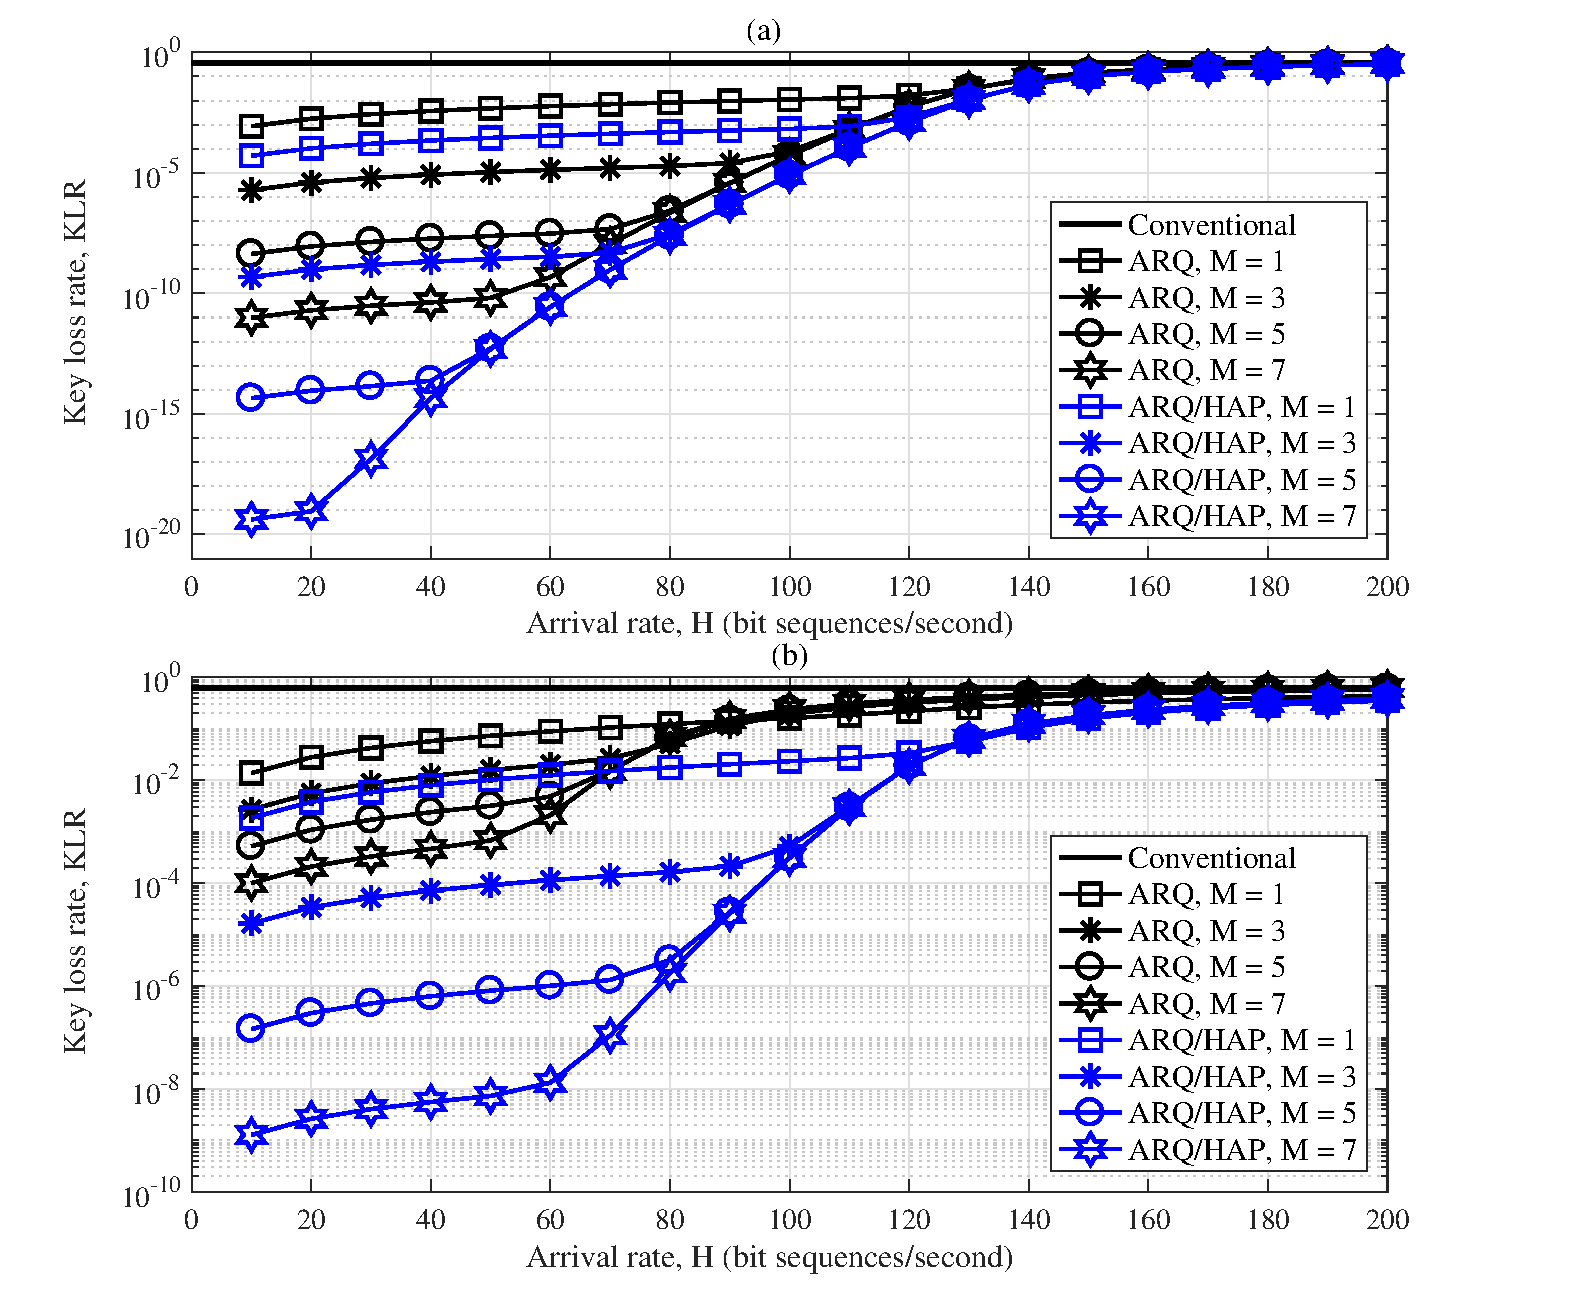
\includegraphics[width=8cm]{Figures/Figure3.eps}
\end{center}
\caption{The key loss rate (KLR) versus arrival rate ($H$) under (a) weak and (b) strong turbulence conditions, when $C=10$ (bit sequences).}
\label{fig:KeyLossRate_ArrivalRate}
\end{figure} 

Figure \ref{fig:KeyLossRate_ArrivalRate} investigates key loss rate (KLR) performance versus arrival rate $H$ under (a) weak and (b) strong turbulence conditions. Firstly, I confirm that the KLR of the conventional system is relatively high, although the satellite's TX telescope gain and ground station's RX one can be respectively boosted to $130$ dB as well as $135$ dB, due to impacts of atmospheric turbulence. KLR can be improved thanks to the use of link-layer ARQ especially when it is combined with HAP-based relaying. The advantage of using the combined technique, i.e., both HAP-based relaying and ARQ, compared to ARQ only can be observed evidently, especially for a higher value of $M$. In Fig. \ref{fig:KeyLossRate_ArrivalRate}(b) with $M=3$ , the maximum arrival rates corresponding to $\textnormal{KLR}=10^{-2}$ are $120$ (sequences/second) for ARQ/HAP case and $50$ (sequences/second) for ARQ case. However, using combined techniques can only improve the KLR performance in the low arrival rate. When the arrival rate reaches a certain level, the use of combined techniques does not bring the advantage due to the probability that Ruby's buffer is full increases. The utilization of combined techniques is recommended when $H < 180$ for both turbulence conditions.

\subsection{Delay Outage Rate}
\begin{figure}[t]
\begin{center}
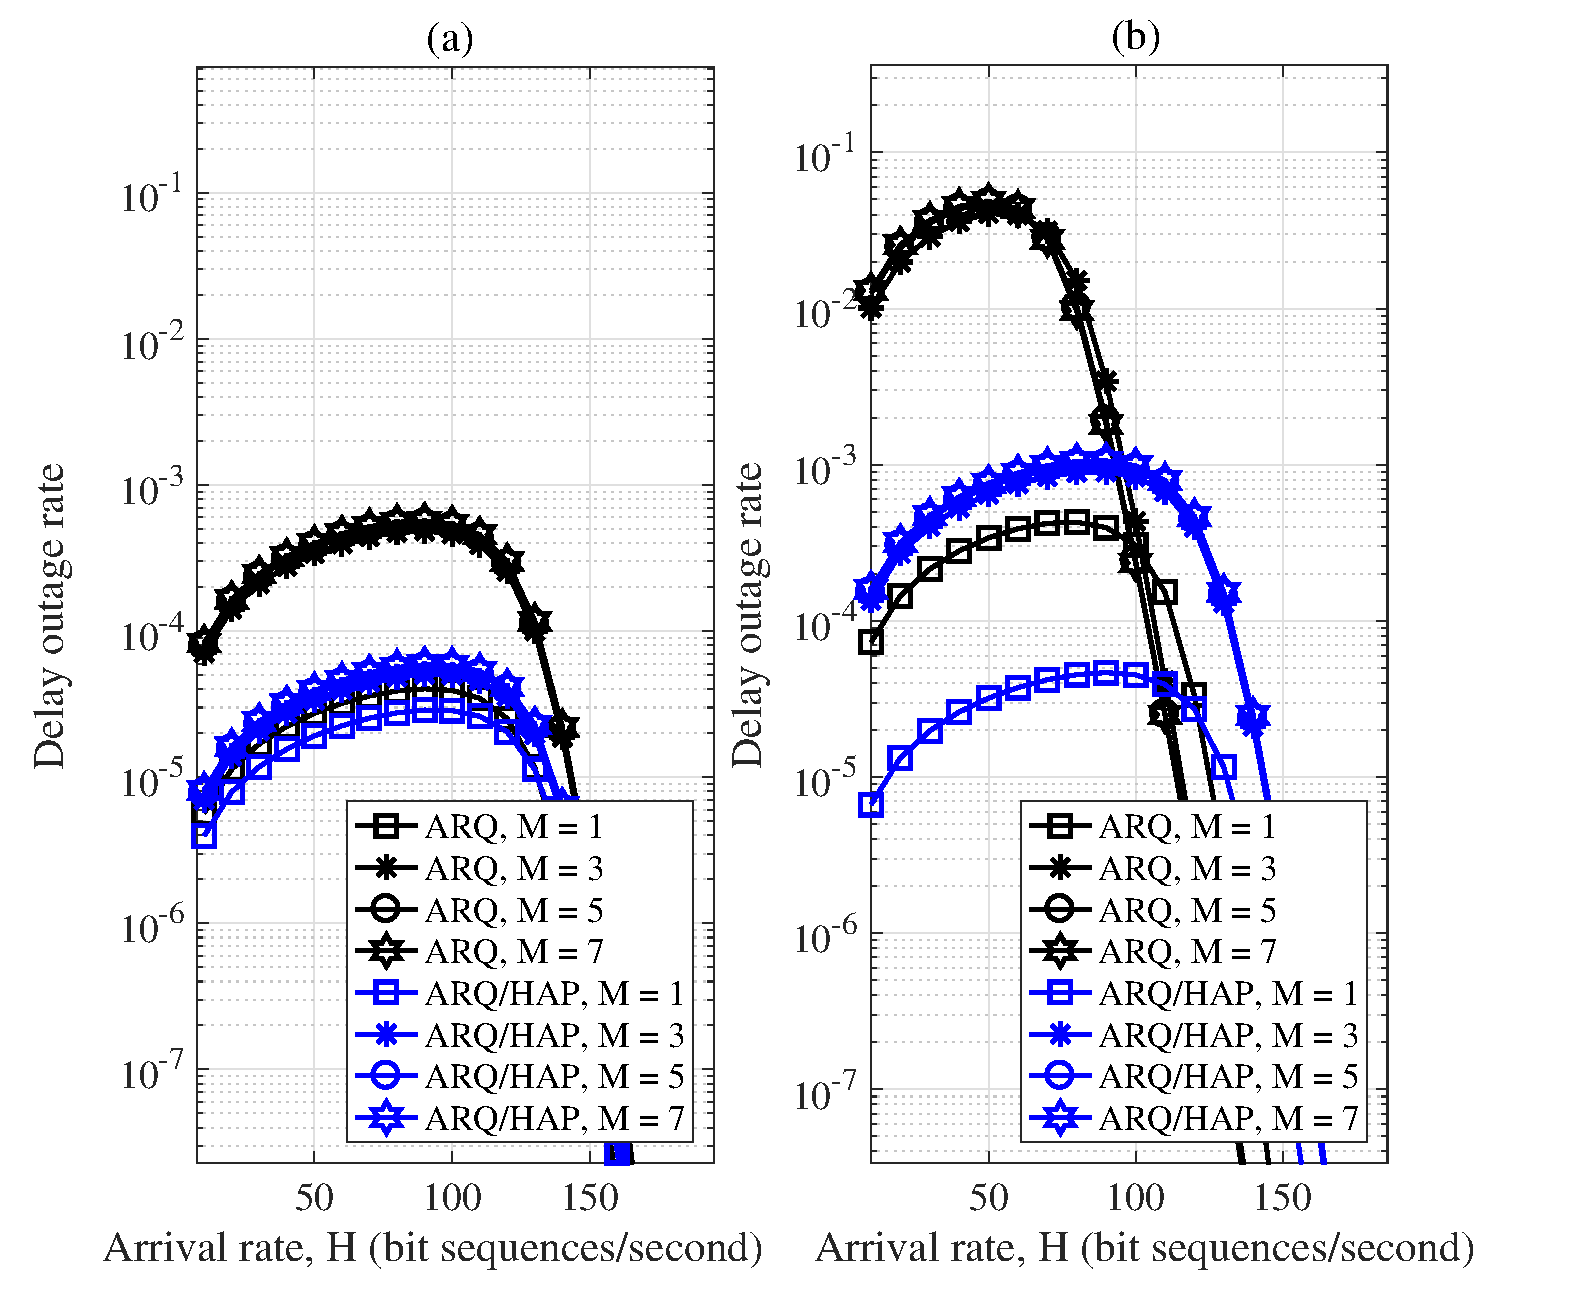
\includegraphics[width=7.5cm]{Figures/Figure4.eps}
\end{center}
\caption{The delay outage rate versus arrival rate ($H$) under (a) weak and (b) strong turbulence conditions, when $C=10$ (sequences).}
\label{fig:DelayOutageRate_ArrivalRate}
\end{figure} 

The delay outage rate versus arrival rate $H$ under different turbulence conditions is considered in Fig. \ref{fig:DelayOutageRate_ArrivalRate}. We can realize the delay outage rate in the case of ARQ/HAP is lower than that of ARQ cases, especially in strong turbulence conditions. This is because HAP-based relaying is an efficient method for reducing the key error rate and thus the number of times required for retransmission, which causes the delay. In addition, the increase of $M$ also causes more delay. 

Figure \ref{fig:DelayOutageRate_ArrivalRate} also shows the delay outage rate clearly varies with the arrival rate. In the beginning, because of a higher arrival rate leads to a higher queuing delay, therefore the delay outage increases with the arrival rate. The delay decreases when the arrival rate reaches a certain level. However, in this case, bit sequences are discarded due to buffer overflow, and hence the ratio of successfully received bit sequences decreases.

Figure \ref{fig:DelayOutageRate_BufferSize} depicts the delay outage rate versus Ruby's buffer size $C$ under turbulence conditions. It is clear that longer buffer size helps to reduce KLR; however, it causes more delay. In order to ensure the delay outage rate below a certain threshold, we need significantly to derive the maximum level of Ruby's buffer size. In the case of ARQ/HAP and strong turbulence conditions, the maximum buffer size is $10$ sequences with the delay outage rate of $10^{-3}$. This value corresponding to different values of $M$ is trivial under weak turbulence conditions, while they are much different under strong turbulence conditions. The reason is that strong turbulence conditions cause high KLR and thus the number of retransmissions has more impact. With the same buffer size, clearly, the delay outage rate is smaller for the case of weak turbulence conditions.

\subsection{Ergodic Secret-Key Rate}
\begin{figure}[t]
\begin{center}
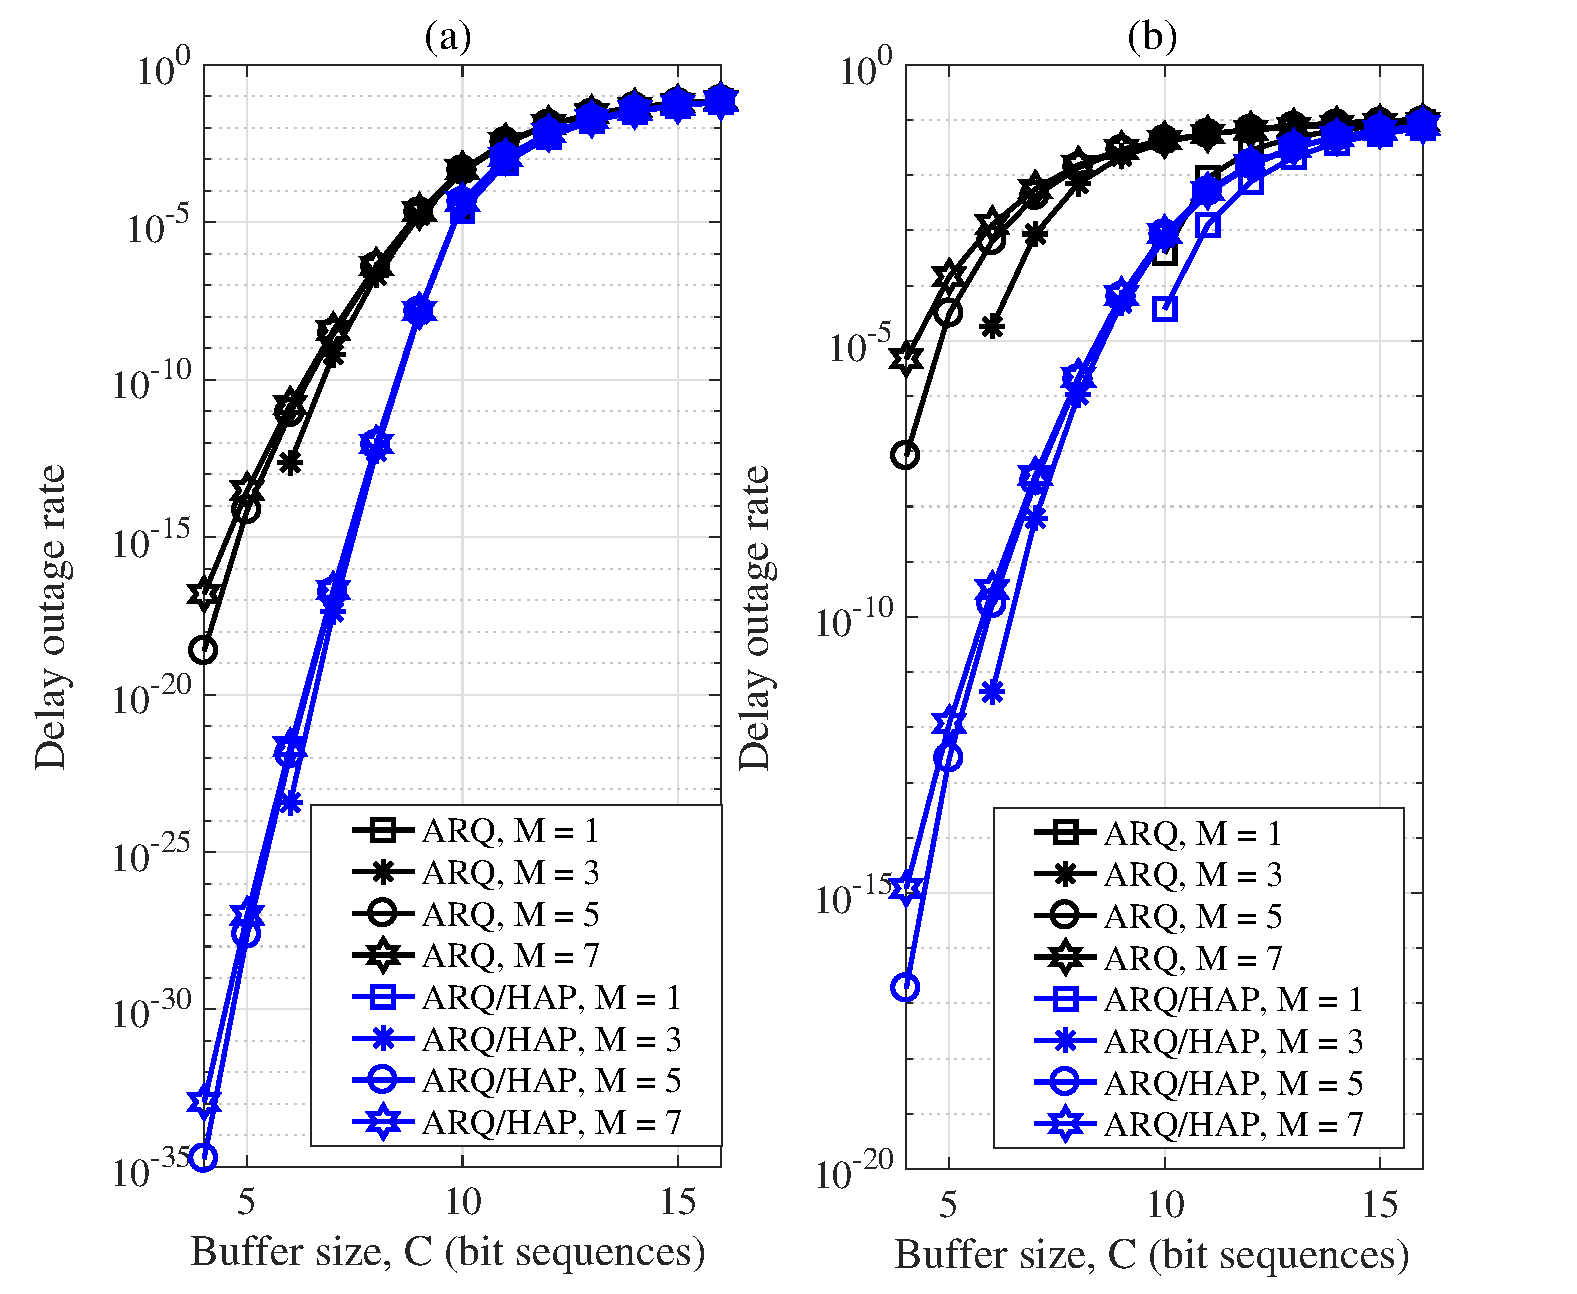
\includegraphics[width=7.5cm]{Figures/Figure5.eps}
\end{center}
\caption{The delay outage rate versus Ruby's buffer size ($C$) under (a) weak and (b) strong turbulence conditions, when $H=60$ (sequences/second).}
\label{fig:DelayOutageRate_BufferSize}
\end{figure} 

\begin{figure}[t]
\begin{center}
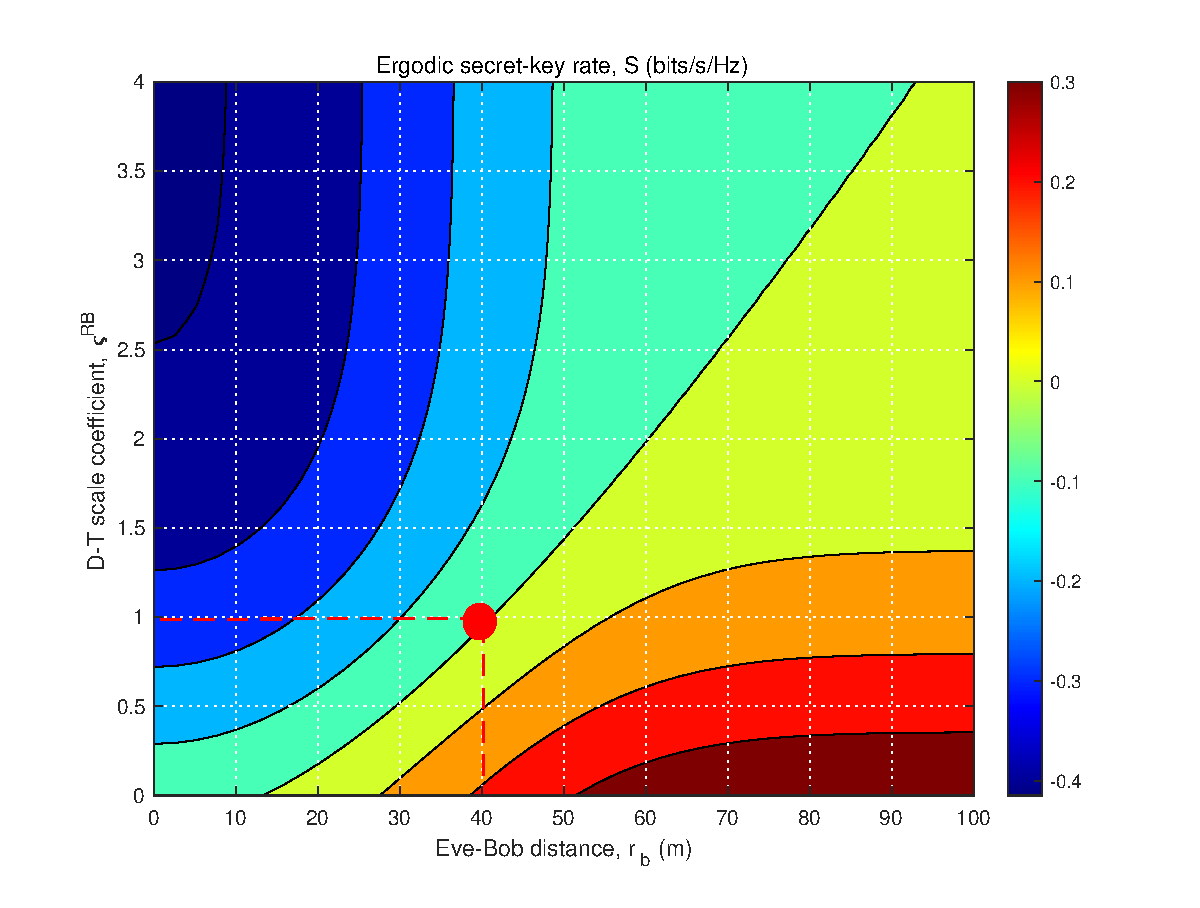
\includegraphics[width=7.5cm]{Figures/Figure6.eps}
\end{center}
\caption{Ergodic secret-key rate ($S$) versus dual threshold (D-T) scale coefficient under strong turbulence condition.}
\label{fig:ErgodicSecretKeyRate}
\end{figure}

Figure \ref{fig:ErgodicSecretKeyRate} shows the ergodic secret-key rate ($S$) versus the distance between Eve and Bob when the D-T scale coefficient can be adjusted by Bob. Obviously, the secret-key rate increases when Eve is far away from Bob. This is due to the reduction of the optical power collected by Eve, therefore, the mutual information between Alice and Eve is decreased. Using this result, we can determine the minimum distance between Eve and Bob which we can guarantee that the proposed QKD system is secured (i.e., $S>0$). For example, when Bob sets D-T scale coefficient $\varsigma^{(RB)}=1$, he can always guarantee a secure channel with Alice whenever Eve is at least $40$ m away from himself.
%=============================================================
\section{Conclusion}\label{sect:Conclusion}
I investigated the use of HAP-based relaying and link-layer ARQ techniques for performance improvement of satellite FSO/QKD systems. We also derived the mathematical expressions for three important performance metrics, the key loss rate, the delay outage rate, and ergodic secret-key rate of the proposed systems. Numerical results showed that the combination of HAP-based relaying and ARQ helps to significantly improve the system performance, especially under strong atmospheric turbulence conditions. Also, the proper values of the arrival rate and the buffer size can be determined so as to the delay outage rate meets a specific requirement. The initial results confirmed the feasibility of  the proposed design in terms of achievable secret-key rate and help to find out suitable parameters for preventing eavesdroppers.

%=============================================================
\begin{thebibliography}{99}
\bibitem{Yuen2016}
H. P. Yuen, 
\enquote{Security of quantum key distribution,}
\emph{IEEE Access,} vol. 4, pp. 724--749, 2016.

\bibitem{Vallone2015}
G. Vallone et. al., 
\enquote{Experimental satellite quantum communications,}
\emph{Phys. Rev. Lett.} 115(4), 040502, 2015.

\bibitem{Liao2018}
S.-K. Liao et. al., 
\enquote{Satellite-relayed intercontinental quantum network,}
\emph{Phys. Rev. Lett.} 120(3), 030501, 2018.

\bibitem{Buttler2003}
W.T. Buttler et. al., 
\enquote{Fast efficient error reconciliation for quantum cryptography,}
\emph{Phys. Rev. A,} vol. 67, No. 5, p. 052303, 2003.

\bibitem{Ai2020}
X. Ai et. al., 
\enquote{A reconciliation strategy for real-time satellite-based QKD,} 
\emph{IEEE Wireless Commun. Lett.,} vol. 24, no. 5, pp. 1062--1066, May 2020. 

\bibitem{MinhVu2019}
Minh B. Vu et. al.,
\enquote{Satellite-based free-space quantum key distribution systems using QPSK modulation and heterodyne detection receiver,}
\emph{2019 19th ISCIT,} Ho Chi Minh City, Vietnam, 2019, pp. 265--270.

\bibitem{Bennett1984}
C. H. Bennett et. al., 
\enquote{Quantum cryptography: public key distribution and coin tossing,}
\emph{Proc. IEEE Int. Conf. Comput. Syst. Signal Process,} Bangalore, India, 1984, pp. 175--179.

\bibitem{Gisin2002}
N. Gisin et. al., 
\enquote{Quantum cryptography,}
\emph{Rev. Modern Phys.,} vol. 74, p. 145, Mar. 2002. 

\bibitem{Trinh2018}
P. V. Trinh et. al.,
\enquote{Design and security analysis of quantum key distribution protocol over free-space optics using dual-threshold direct-detection receiver,}
\emph{IEEE Access,} vol. 6, pp. 4159--4175, 2018.

\bibitem{Vu2019}
M. Q. Vu et. al., 
\enquote{HAP-aided relaying satellite FSO/QKD systems for secure vehicular networks,}
\emph{2019 IEEE 89th VTC2019-Spring,} Kuala Lumpur, Malaysia, 2019.

\bibitem{Shen2006}
H. Shen et. al., 
\enquote{Performance analysis of TFRC over wireless link with truncated link-level ARQ,}
\emph{IEEE Trans. Wirel. Commun.,} vol. 5, no. 6, pp. 1479--1487, June 2006.

\end{thebibliography}
\end{document}